\documentclass[10pt]{beamer}

\usepackage{booktabs}
\usepackage{setspace}
\usepackage{amsmath}
\usepackage{amssymb}
\usepackage{latexsym}
\usepackage{epsfig}
\usepackage{listings}
\usepackage{url}
\usepackage{epsfig}
\usepackage{fancybox}
\usepackage{graphicx} 
\usepackage{color}
\usepackage{subfigure}

% Theme
\usetheme{Berlin}
\usecolortheme{whale}
\useoutertheme{infolines}
\useinnertheme{circles}
%\usefonttheme[onlymath]{structurebold}
%\usefonttheme{professionalfonts}
\setbeamertemplate{blocks}[rounded][shadow=true]
\setbeamertemplate{navigation symbols}{-}

% support algorithm and pseudocode
\usepackage{algorithm, algorithmic}
\renewcommand{\algorithmicrequire}{\textbf{Input:}}
\renewcommand{\algorithmicensure}{\textbf{Output:}}

% set the color of every meth formular to blue
\everymath{\color{blue}}

% listing set
\definecolor{lightlightgray}{gray}{0.9}
\lstset{ %
language=Octave,                % the language of the code
basicstyle=\ttfamily\small\bfseries,       % the size of the fonts that are used for the code
keywordstyle=\color{blue!100},   % color of the keyword
commentstyle=\color{red!50!green!50!blue!50},
rulesepcolor=\color{red!20!green!20!blue!20},escapeinside=``,
xleftmargin=2em,
xrightmargin=2em,
aboveskip=1em,
numbers=left,                   % where to put the line-numbers
numberstyle=\tiny,              % the size of the fonts that are used for the line-numbers
stepnumber=1,                   % the step between two line-numbers. If it's 1, each line will be numbered
numbersep=5pt,                  % how far the line-numbers are from the code
backgroundcolor=\color{lightlightgray},  % choose the background color. You must add \usepackage{color}
showspaces=false,               % show spaces adding particular underscores
showstringspaces=false,         % underline spaces within strings
showtabs=false,                 % show tabs within strings adding particular underscores
frame=shadowbox,                % adds a frame around the code
tabsize=2,                      % sets default tabsize to 2 spaces
captionpos=b,                   % sets the caption-position to bottom
breaklines=true,                % sets automatic line breaking
breakatwhitespace=false,        % sets if automatic breaks should only happen at whitespace
title=\lstname,                 % show the filename of files included with \lstinputlisting;
                                % also try caption instead of title
escapeinside={\%*}{*)},         % if you want to add a comment within your code
morekeywords={*,...}            % if you want to add more keywords to the set
}

% Set the basic info of the presentation
\title[CLCS]{Computing the Length of Constraint Longest Common Subsequence}
\author[B.Yu \and W.Sun \and B.Zhu \and W.Sha]{Bai Yu \and Wukong Sun \and Bajie Zhu \and Wujing Sha}
\institute[ZJU]{
  Mathematical and Computer Sciences and Engineering Division\\
  Zhejiang University, China\\
}
\date{\today}
\begin{document}

%----------- titlepage ----------------------------------------------%
\begin{frame}[plain]
  \titlepage
%  Presenter: Bai Yu \url{zjuyubai@gmail.com}
\end{frame}

\section[outline]{}
%----------- slide --------------------------------------------------%
\begin{frame}
  \frametitle{Outline}
  \tableofcontents
\end{frame}

\section{Brief Introduction to the Problem}
%----------- slide --------------------------------------------------%
\begin{frame}[fragile]
  \frametitle{Brief Introduction to the Problem} 
\begin{definition}[\textbf{CLCS}]
  The \alert{\texttt{Constraint Longest Common Subsequence (CLCS)}} problem is to find the longest subsequence common to all the given strings with respect to the constraint sequence. Thus, given two strings $X$, $Y$,  and a contraint string $P$,  find the longest common subsequence $Z$ of $X$ and $Y$ such that $P$ is a subsequence of $Z$.
\end{definition}

\vskip10pt
\pause

\begin{example}
For example, given input $X="abc123"$, $Y="123abc"$, and $P="ab"$, the LCS of $X$ and $Y$ is $"abc"$ and $"123"$, while the {\structure{CLCS}} with respect to $P$ is $"abc"$.
\end{example}

\end{frame}

\section{Algorithms Description}
%----------- slide --------------------------------------------------%
\begin{frame}
  \frametitle{Algorithms Description}

  \begin{itemize}
    \item<1-> Algorithms

  We use the algorithms by \emph{Yin-Te Tsai} and by \emph{Francis Chin, et al.} to solve this problem.

    \vskip15pt

    \item<2-> Time complexity

  Assume the lengths of $X$, $Y$ and $P$ be $n$, $m$ and $r$ respectively. 
  \begin{itemize}
    \item Tsai's algorithm solves the problem in $O(n^2m^2 r)$ time.
    \item Chin's algorithm in $O(nmr)$ time.
  \end{itemize}

    \vskip15pt
    \item<3-> Technique

    Dynamic Programming

  \end{itemize}

\end{frame}

\subsection{Algorithm by Yin-Te Tsai}
%----------- slide --------------------------------------------------%
\begin{frame}
  \frametitle{Algorithm by Yin-Te Tsai}
  Let $L(x, y, x^{\prime}, y^{\prime})$ denotes the length of LCS of strings $X[x..x^{\prime}]$ and $Y[y..y^{\prime}]$.

  Let $L_k (i, j )$ denotes the length of  CLCS of strings $X[1..i]$ and $Y[1..j ]$ w.r.t $P[1..k]$.

  \pause
\begin{proof}[\textbf{Recursive Relation}]
  For  $1\le i \le n$ , $1\le j\le m$ and $1\le k \le r$, $L_1(i, j ) = L(1, 1, i -1, j -1)+1$ if $X[i] = Y[j] = P[1]$, and $-\infty$ otherwise. 

  For $2\le k \le r$, $1\le i \le n$, and $1\le j \le m$, 
  {\footnotesize{
      \begin{equation}\label{eq:Lk}
        L_k(i, j) = \left\{
	\begin{array}{ll}
	  \max\{L_{k-1}(x,y), L(x+1, y+1, i-1, j-1) + 1\} & \textrm{if} X[i]=Y[j]=P[k];\\
          -\infty & \textrm{otherwise}
	\end{array}
	\right. 
      \end{equation}
    }
  }
\end{proof}

  \pause
  After obtaining $L_k(\cdot, \cdot)$, we compute the length of CLCS with the following formula:
  \begin{equation}\label{eq:z}
    |Z| = \max_{1\le i\le n, 1\le j\le m} \{L_r(i, j) + L(i+1, j+1, n, m) \}
  \end{equation}

\end{frame}

%----------- slide --------------------------------------------------%
\begin{frame}
  \frametitle{Algorithm by Yin-Te Tsai}

\pause
Time:

\begin{itemize}
  \item<3-> Pre-computation of $L$: $O(n^2m^2)$
  \item<4-> Compute all the $L_k$: $O(n^2m^2r)$
  \item<5-> Compute $|Z|$ from $L_k$ to $L$: $O(nm)$
  \item<6-> Total: $O(n^2m^2)$ + $O(n^2m^2r)$ + $O(nm)$ = $O(n^2m^2r)$
\end{itemize}

\vskip15pt

\pause\pause\pause\pause\pause
Space:

\begin{itemize}
  \item<8-> Space for $L(.,.,.,.)$: $O(n^2m^2)$
  \item<9-> Space for $L_k(.,.)$: $O(nmr)$
  \item<10-> Total: $O(n^2m^2)$ + $O(nmr)$ = $O(n^2m^2)$
\end{itemize}

\end{frame}

%----------- slide --------------------------------------------------%
\begin{frame}
  \frametitle{Algorithm by Yin-Te Tsai}

Example: $X=``aba"$, $Y=``bab"$, $P=``a"$.

\begin{table}[ht]
\centering
\subtable{
       \begin{tabular}{|c|c|c|c|c|}
		\hline
		$M_{1,1}$ &   & b & a & b\\ \hline
		          & 0 & 0 & 0 & 0\\ \hline
		a         & 0 & 0 & 1 & 1\\ \hline
		b         & 0 & 1 & 1 & 2\\ \hline
		a         & 0 & 1 & 2 & 2\\
		\hline
	\end{tabular}
}
\quad
\subtable{        
       \begin{tabular}{|c|c|c|c|}
		\hline
		$M_{1,2}$ &   & a & b\\ \hline
		          & 0 & 0 & 0\\ \hline
		a         & 0 & 1 & 1\\ \hline
		b         & 0 & 1 & 2\\ \hline
 		a         & 0 & 1 & 2\\
		\hline
		\end{tabular}
}
\quad
\subtable{
	\begin{tabular}{|c|c|c|}
		\hline
		$M_{1,3}$ &   & b\\ \hline
		          & 0 & 0\\ \hline
		a         & 0 & 0\\ \hline
		b         & 0 & 1\\ \hline
		a         & 0 & 1\\
		\hline
	\end{tabular}
}\\
\subtable{
       \begin{tabular}{|c|c|c|c|c|}
		\hline
		$M_{2,1}$ &   & b & a & b\\ \hline
		          & 0 & 0 & 0 & 0\\ \hline
		b         & 0 & 1 & 1 & 1\\ \hline
		a         & 0 & 1 & 2 & 2\\
		\hline
	\end{tabular}
}
\quad
\subtable{
       \begin{tabular}{|c|c|c|c|}
		\hline
		$M_{2,2}$ &   & a & b\\ \hline
		          & 0 & 0 & 0\\ \hline
		b         & 0 & 0 & 1\\ \hline
		a         & 0 & 1 & 1\\
		\hline
	\end{tabular}
}
\quad
\subtable{
       \begin{tabular}{|c|c|c|}
		\hline
		$M_{2,3}$ &   & b\\ \hline
		          & 0 & 0\\ \hline
		b         & 0 & 1\\ \hline
		a         & 0 & 1\\
		\hline
	\end{tabular}
}\\
\subtable{
       \begin{tabular}{|c|c|c|c|c|}
		\hline
		$M_{3,1}$ &   & b & a & b\\ \hline
		          & 0 & 0 & 0 & 0\\ \hline
		a         & 0 & 0 & 1 & 1\\
		\hline
	\end{tabular}
}
\quad
\subtable{
       \begin{tabular}{|c|c|c|c|}
		\hline
		$M_{3,2}$ &   & a & b\\ \hline
		          & 0 & 0 & 0\\ \hline
		a         & 0 & 1 & 1\\
		\hline
	\end{tabular}
}
\quad
\subtable{
       \begin{tabular}{|c|c|c|}
		\hline
		$M_{3,3}$ &   & b\\ \hline
		          & 0 & 0\\ \hline
		a         & 0 & 0\\
		\hline
	\end{tabular}
}
\end{table}

\end{frame}


%----------- slide --------------------------------------------------%
\begin{frame}
  \frametitle{Algorithm by Yin-Te Tsai}
Example: $X=``aba"$, $Y=``bab"$, $P=``a"$.

Then we compute states $L_k(i,j)$.

\begin{enumerate}
	\item<2-> ($X[1]\neq Y[1]$) $L_{1}(1,1) = -\infty$;
	\item<3-> ($X[1]=Y[2]=P[1]$) $L_{1}(1,2)=L(1,1,0,1) + 1 = 1$;
	\item<4-> ($X[1]\neq Y[3]$) $L_{1}(1,3)=-\infty$;
	\item<5-> ($X[2]=Y[1]\neq P[1]$) $L_{1}(2,1) = -\infty$;
	\item<6-> ($X[2]\neq Y[2]$) $L_{1}(2,2)=-\infty$;
	\item<7-> ($X[2]=Y[3]\neq P[1]$) $L_{1}(2,3)=-\infty$;
	\item<8-> ($X[3]\neq Y[1]$) $L_{1}(3,1)=-\infty$;
	\item<9-> ($X[3]=Y[2]=P[1]$) $L_{1}(3,2) = L(1,1,2,1) +1 = 2$;
	\item<10-> ($X[3]\neq Y[3]$) $L_{1}(3,3)=-\infty$.
\end{enumerate}

\pause\pause\pause\pause\pause\pause\pause\pause\pause\pause

Finally, we compute the length of CLCS: 
\[|Z| = \max_{1\le i\le 3, 1\le j\le 3} \{L_{1}(i,j)+L(i+1, j+1, 3,3)\}=2\]

\end{frame}

\subsection{Algorithm by Francis Chin et al.}
%----------- slide --------------------------------------------------%
\begin{frame}
  \frametitle{Algorithm by Francis Chin et al.}
  Given two  strings $X$, $Y$ of length $n$, $m$ respectively, and  a contraint string $P$ of length $r$, we define $L(i, j, k)$ as the CLCS length of $X[1..i]$,  $Y[1..j]$ w.r.t $P[1..k]$.

  \pause
  \begin{proof}[Recursive Relation]
    For any $0\le i \le n$, $0\le j\le m$ and $0\le k \le r$:
    {\scriptsize{
        \begin{equation}\label{eq:recur}
          L(i,j,k)=\left\{
          \begin{array}{ll}
            1+ L(i-1, j-1, k-1) & \textrm{if } i, j, k > 0 \textrm{ and } X[i]= Y[j] = P[k]\\
            1+ L(i-1, j-1, k)    & \textrm{if } i, j > 0, X[i]=Y[j] \textrm{ and } (k=0 \textrm{ or } X[i]\neq P[k])\\
            \max(L(i-1, j, k), L(i, j-1, k)) & \textrm{if } i, j > 0 \textrm{ and } X[i]\neq Y[j]
          \end{array}
          \right.
        \end{equation}
      }
    }
    with boundary conditions, $L(i, 0, 0)=L(0, j, 0)=0$ and $L(0, j, k)= L(i, 0, k)=-\infty$ for any $0\le i \le n$, $0\le j\le m$ and $0< k \le r$.
  \end{proof}
  
  \vskip10pt
  \pause
  The length of CLCS of $X$, $Y$ with respect to $P$ is given by $L(n,m,r)$. 

\end{frame}

%----------- slide --------------------------------------------------%
\begin{frame}
  \frametitle{Algorithm by Francis Chin}
  From the equation $(3)$, the recursive relation of Chin's algorithm, we can use recursive backtracking from the relations to analysis the complexity of this algorithm.

  \vskip10pt
  \pause
  From analysis of the computation path, we know that it takes at most $O(n + m + r)$ steps.And we can also say that it takes $O(n*m*r)$ time and space to build and calculate the constraint longest common sequence.
  
\end{frame}

%----------- slide --------------------------------------------------%
\begin{frame}
  \frametitle{Algorithm by Francis Chin}
  Example: $X=``aba"$, $Y=``bab"$, $P=``a"$.

  \begin{enumerate}
  \item<2-> (Boundary states) $L(i,0,0)=L(0,j,0)=0$ for $0\le i\le 3$, $0\le j\le 3$;
    $L(0, j, k)=L(i,0,k)=-\infty$ for $0\le i\le 3$, $0\le j\le 3$, $0<k\le1$;
  \item<3-> ($X[1]\neq Y[1]$) $L(1,1,0)=\max\{L(0,1,0), L(1,0,0)\}=0$;\\
    $L(1,1,1)=\max\{L(0,1,1), L(1,0,1)\}=0$ ;
  \item<4-> ($X[1]=Y[2], k=0$) $L(1,2,0)=1+L(0,1,0)=1$;\\
    ($X[1]=Y[2]=P[1]$) $L(1,2,1)=1+L(0,1,0)=1$;
  \item<5-> ($X[1]\neq Y[3]$) $L(1,3,0)=\max\{L(0,3,0), L(1,2,0)\} = 1$;\\ $L(1,3,1)=\max\{L(0,3,1), L(1,2,1)\}=1$;
  \item<6-> ($X[2]=Y[1], k=0$) $L(2,1,0) = 1+ L(1,0,0) = 1$; \\
    ($X[2]=Y[1]\neq P[1]$) $L(2,1,1)=1+L(1,0,1)=-\infty$;
  \end{enumerate}
\end{frame}

%----------- slide --------------------------------------------------%
\begin{frame}
  \frametitle{Algorithm by Francis Chin}
  Example: $X=``aba"$, $Y=``bab"$, $P=``a"$.

  \begin{enumerate}
  \addtocounter{enumi}{5}
  \item<2-> ($X[2]\neq Y[2]$) $L(2,2,0) = \max\{L(1,2,0), L(2,1,0)\}=1$;\\ $L(2,2,1)=\max\{L(1,2,1),L(2,1,1)\}=1$;
  \item<3-> ($X[2]=Y[3], k=0$) $L(2,3,0)=1+L(1,2,0) = 2$; \\
    ($X[2]=Y[3]\neq P[1]$) $L(2,3,1) =1+\max\{L(1,3,1),L(2,2,1)\}=2$
  \item<4-> ($X[3]\neq Y[1]$) $L(3,1,0)=\max\{L(2,1,0), L(3,0,0)\}=1$;\\ $L(3,1,1)=\max\{L(2,1,1), L(3,0,1)\}=-\infty$;
  \item<5-> ($X[3]=Y[2], k=0$) $L(3,2,0)=1+ L(2,1,0) = 2$;\\
    ($X[3]=Y[2]=P[1]$) $L(3,2,1)=1+L(2,1,0) = 2$;
  \item<6-> ($X[3]\neq Y[3]$) $L(3,3,0) = \max\{L(2,3,0), L(3,2,0)\} = 2$;\\ $L(3,3,1) = \max\{L(3,2,1), L(2,3,1)\}=2$.
  \end{enumerate}

  \pause\pause\pause\pause\pause\pause
  Finally, $|Z|=L(3,3,1)=2$.

\end{frame}

\section{Experimental Study}
%----------- slide --------------------------------------------------%
\begin{frame}
  \frametitle{Experimental Study}
We took two steps to perform this study. 
  \begin{enumerate}
    \item<1-> \textbf{Correctness}

First we implemented the algorithms and tested the correctness of implementation with manually selected test cases and program-generated test cases. 
    \item<2-> \textbf{Performance}

Then we ran the programs with large program-generated test cases to assess the performance.
  \end{enumerate}
\end{frame}

\subsection{Correctness}
%----------- slide --------------------------------------------------%
\begin{frame}
  \frametitle{Correctness}
To test whether the algorithms were correctly implemented, we chose a few boundary cases to do white-box test, and generated a series of test cases for black-box test.

  \medskip
  \medskip

The program-generated test cases consist of all the possible combinations of the strings of length less than four. We have $39^3=59319$ different test cases. 

  \medskip
  \medskip

As the test cases are regularly generated, it is easy to manually find out the answers to the cases. 

\end{frame}

\subsection{Performance}
%----------- slide --------------------------------------------------%
\begin{frame}
  \frametitle{Performance}
Randomly generated a series of 3-tuples as test cases. Each tuple consists of two strings and a constraint string, which are defined on the alphabet $\Sigma=\{A,T,G,C\}$. 
For the $k$-th tuple $(X,Y,P)$, the lengths of the elements satisfy the condition $|X|=|Y|=2|P| = 10k$. 
\begin{center}
\begin{figure}[ht]
	\centering
	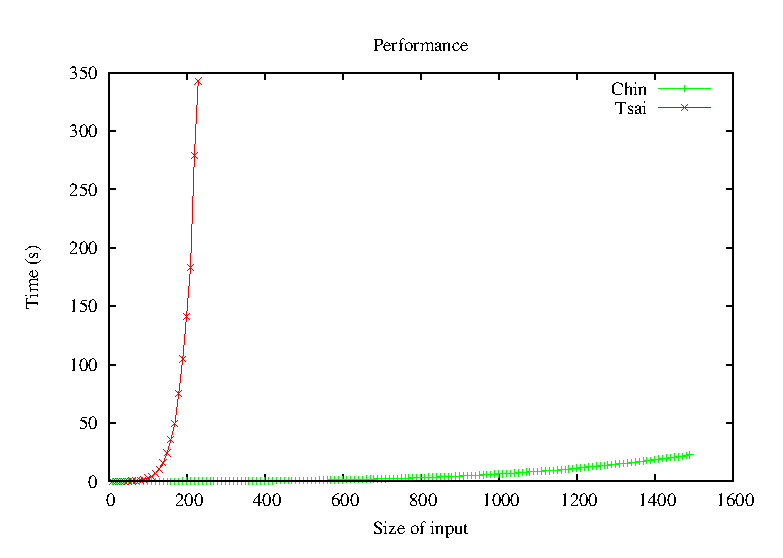
\includegraphics[scale=0.55]{images/experiment.eps}
%	\caption{}\label{fig:test}
\end{figure}
\end{center}
\end{frame}

\section{Fitting Data with Polynomials}
\subsection[Chin's algorithm]{}
%----------- slide --------------------------------------------------%
\begin{frame}
  \frametitle{Fitting Data with Polynomials}
Chin's algorithm
\begin{center}
\begin{figure}[ht]
	\centering
	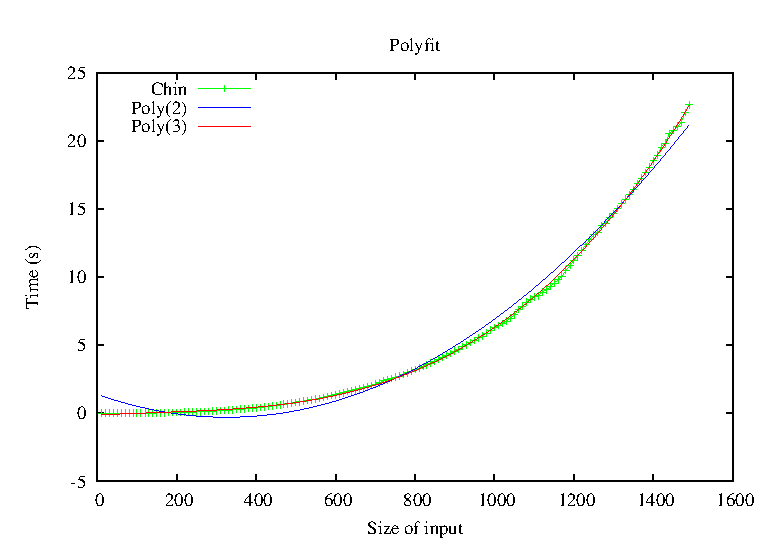
\includegraphics[scale=0.7]{images/polyfit-chin.eps}
%	\caption{}\label{fig:test}
\end{figure}
\end{center}
\end{frame}

\subsection[Tsai's algorithm]{}
%----------- slide --------------------------------------------------%
\begin{frame}
  \frametitle{Fitting Data with Polynomials}
Tsai's algorithm
\begin{center}
\begin{figure}[ht]
	\centering
	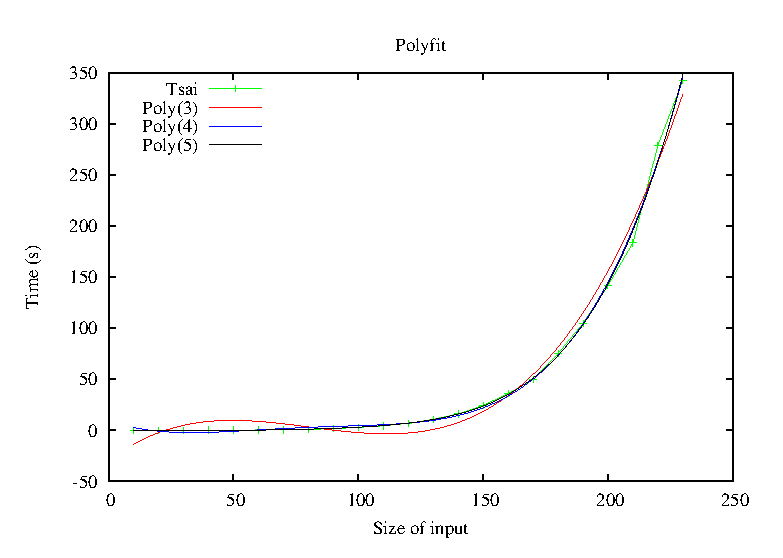
\includegraphics[scale=0.7]{images/polyfit-tsai.eps}
%	\caption{}\label{fig:test}
\end{figure}
\end{center}
\end{frame}

\section[References]{}
%----------- slide --------------------------------------------------%
\begin{frame}
  \frametitle{References}
% This includes all references from the BibTeX file in the bibliography
\nocite{*}
\begin{spacing}{1}
  \bibliographystyle{unsrt}
  \bibliography{bib/bibtexDB}
\end{spacing}
\end{frame}

\end{document}
